\chapter{SparkContext的初始化}
\label{scinitial}
Driver线程启动子线程来加载用户程序主类,主类中第一步是对SparkContext的初始化,SparkContext可以算得上是所有用户程序的启动引擎。而SparkContext初始化的配置参数由SparkConf负责。
\section{执行环境SparkConf}
SparkConf的构造很简单,主要包含的是提交用户程序的参数信息,包括setMaster、setAppName等。Spark的配置属性都是以“Spark.”开头的字符串。下面介绍SparkConf中重要的方法
\begin{enumerate}[\bfseries 1]
	\item registerKryoClasses
	
	注册时使用Kryo序列化的类,指定该类的序列化器为Kryo,关于Kryo的使用是spark性能优化的一个重要的组成部分。其中一个简单的应用是图计算。
	\item registerAvroSchemas
	
	序列化前先对Schema进行注册,影响的是压缩效率。
\end{enumerate}
\section{SparkContext综合概述}
配置完的SparkConf传入SparkContext,将SparkContext比作汽车发动机的引擎,SparkConf就是我们的控制面板,SparkContext中的SparkEnv创建一些Spark应用运行必备的组件,像Rpc、序列化器、块管理器、缓存管理器、测量系统、中间数据追踪器及文件服务器等,可以理解为汽车的空调、电路、油门线等环境条件。SparkContext和SparkEnv关系可以表示为
\tcbset{colback=red!5!white,colframe=red!75!black}
\tcbsetforeverylayer{colframe=red!75!black}
\begin{tcolorbox}[title=SparkContect]
	\begin{tabularx}{\linewidth}{XXXX}
		callSite&listenerBus&\_metadataCleaner&\_statusTracker\\
		SparkUI&\_dagScheduler&\_schedulerBackend&\_taskScheduler\\
	\end{tabularx}
	\begin{tcolorbox}[title=SparkEnv]
		\begin{tabularx}{\linewidth}{XXX}
			RpcEnv&serializer&closureSerializer\\
			mapOutputTracker&shuffle类型&blockManager(master)\\
			broadcastManager&cacheManager&metricsSystem\\
		\end{tabularx}
	\end{tcolorbox}
\end{tcolorbox}
\subsection{调用栈}
CallSite中存储了线程栈中最靠近栈顶的用户类以及最靠近栈底的Scala或者Spark核心类,这个变量其实主要是给开发者看的,对于具体程序的运行没有必然的影响。当然它的信息也会反应在SparkUI的界面上的。
\subsection{监听主线ListenerBus}
Spark消息系统的具体实现为后台会自动开启一个线程来监听事件,现在基本上所有的分布式系统都是通过消息驱动的方式来进行并发执行的。具体的线程执行如程序\ref{inputPrg:listenerThread}所示,从源码中可以看出,它其实是一个守护进程,是通过一个死循环,对事件队列里所有的事件进行遍历,再将不同的事件发送给不同的监听器Listener。
\begin{codeInput}{Scala}{listenerBus程序代码片段}{listenerThread}
private val listenerThread = new Thread(name) {
  setDaemon(true)
  override def run(): Unit = Utils.tryOrStopSparkContext(sparkContext) {
    AsynchronousListenerBus.withinListenerThread.withValue(true) {
      while (true) {
        eventLock.acquire()
          self.synchronized {
            processingEvent = true
          }
        try {
          val event = eventQueue.poll
          if (event == null) {
            if (!stopped.get) {
              ......
            }
            return
          }
          postToAll(event)
        } finally {
          self.synchronized {
            processingEvent = false
          }
        }
      }
    }
  }
}
\end{codeInput}
\subsection{元数据清理器}
SparkContext中\_metadataCleaner为元数据清理器,SparkContext为了保持对所有持久化的RDD的跟踪,使用类型是TimeStampped-WeakValueHashMap的persistentRdds缓存。元数据清理器的功能就是清除过期的持久化的RDD。
\subsection{可视化监控服务SparkUI}
Spark UI提供监控功能,以具有样式和布局的网页形式来提供丰富的监控数据,通过浏览器就能进行访问。SparkUI的创建代码如程序\ref{inputPrg:sparkui}所示
\begin{codeInput}{Scala}{SparkUI声明}{sparkui}
    _ui =
    if (conf.getBoolean("spark.ui.enabled", true)) {
      Some(SparkUI.createLiveUI(this, _conf, listenerBus, _jobProgressListener,
      _env.securityManager, appName, startTime = startTime))
    } else {
      // For tests, do not enable the UI
      None
    }
    _ui.foreach(_.bind())
\end{codeInput}
这其中的createLiveUI,实际是调用了SparkUI\#create方法,create方法如程序\ref{inputPrg:sparkcreate}所示
\begin{codeInput}{Scala}{SparkUI创建方法}{sparkcreate}
private def create(
  sc: Option[SparkContext],
  conf: SparkConf,
  listenerBus: SparkListenerBus,
  securityManager: SecurityManager,
  appName: String,
  basePath: String = "",
  jobProgressListener: Option[JobProgressListener] = None,
  startTime: Long): SparkUI = {
    val _jobProgressListener: JobProgressListener = jobProgressListener.getOrElse {
    val listener = new JobProgressListener(conf)
    listenerBus.addListener(listener) listener
  }
  val environmentListener = new EnvironmentListener
  val storageStatusListener = new StorageStatusListener
  val executorsListener = new ExecutorsListener(storageStatusListener)
  val storageListener = new StorageListener(storageStatusListener)
  val operationGraphListener = new RDDOperationGraphListener(conf)	
  listenerBus.addListener(environmentListener)
  listenerBus.addListener(storageStatusListener)
  listenerBus.addListener(executorsListener)
  listenerBus.addListener(storageListener)
  listenerBus.addListener(operationGraphListener)		
  new SparkUI(sc, conf, securityManager, environmentListener, storageStatusListener,
  executorsListener, _jobProgressListener, storageListener, operationGraphListener,
  appName, basePath, startTime)
}
\end{codeInput}

可以看出这里除了JobProgressListener是外部传入的之外,又增加了SparkListener。最后创建SparkUI,SparkUI服务默认是可以被杀掉的,可以修改属性spark.ui.killEnabled为false可以保证不被杀死。类SparkUI构造方法通过调用initialize方法会组织前端各个Tab和Page的展示及布局。
SparkUI的页面布局和展示使用的是JobsTab。它可以展示所有的Job进度、状态信息,这里我们以它为例,JobsTab会复用SparkUI的killEnabled、SparkContext、jobProgressListener,包括AllJobsPage和JobPage两个页面,JobsTab类实现代码程序\ref{inputPrg:jobstab}所示
\begin{codeInput}{Scala}{SparkUI JobsTab}{jobstab}
private[ui] class JobsTab(parent: SparkUI) extends SparkUITab(parent, "jobs") {
  val sc = parent.sc
  val killEnabled = parent.killEnabled
  val jobProgresslistener = parent.jobProgressListener
  val executorListener = parent.executorsListener
  val operationGraphListener = parent.operationGraphListener		
  def isFairScheduler: Boolean =
    jobProgresslistener.schedulingMode.exists(_ == SchedulingMode.FAIR)	
      attachPage(new AllJobsPage(this))
      attachPage(new JobPage(this))
  }
\end{codeInput}

第一个就是AllJobsPage,它由render方法进行渲染,利用jobProgressListener中统计监控数据生成激活、完成、失败等状态Job摘要信息,并调用jobsTable方法生成html各元素,最终使用UIUtils的headerSparkPage封装好css、js、header及页面布局等。 渲染方法部分代码如程序\ref{inputPrg:render}所示
\begin{codeInput}{Scala}{渲染方法实现}{render}
def render(request: HttpServletRequest): Seq[Node] = {
  progressListener.synchronized {
    ......
    val stageHeader = s"Details for Stage $stageId (Attempt $stageAttemptId)"
    if (stageDataOption.isEmpty) {
      val content =
      <div id="no-info">
      <p>No information to display for Stage {stageId} (Attempt {stageAttemptId})</p>
      </div>
      return UIUtils.headerSparkPage(stageHeader, content, parent)	
    }
    if (stageDataOption.get.taskData.isEmpty) {
      val content =
      <div>
      <h4>Summary Metrics</h4> No tasks have started yet
      <h4>Tasks</h4> No tasks have started yet
      </div>
      return UIUtils.headerSparkPage(stageHeader, content, parent)
  }	
  val stageData = stageDataOption.get
  val tasks = stageData.taskData.values.toSeq.sortBy(_.taskInfo.launchTime)
  val numCompleted = tasks.count(_.taskInfo.finished)
  val allAccumulables = progressListener.stageIdToData((stageId, stageAttemptId)).accumulables
  val externalAccumulables = allAccumulables.values.filter { acc => !acc.internal }
  val hasAccumulators = externalAccumulables.size > 0			
  val summary =
  <div>
  <ul class="unstyled">
  <li>
  <strong>Total Time Across All Tasks: </strong>
  {UIUtils.formatDuration(stageData.executorRunTime)}
  </li>
  <li>
  <strong>Locality Level Summary: </strong>
  {getLocalitySummaryString(stageData)}
  </li>
  ......
\end{codeInput}

SparkUI创建好后,需要调用父类的WebUI的bind方法,绑定服务和端口,绑定实现代码如程序\ref{inputPrg:bindsparkui}所示
\begin{codeInput}{Scala}{SparkUI绑定实现}{bindsparkui}
  /** Bind to the HTTP server behind this web interface. */
  def bind() {
    assert(!serverInfo.isDefined, "Attempted to bind %s more than once!".format(className))
    try {
      var host = Option(conf.getenv("SPARK_LOCAL_IP")).getOrElse("0.0.0.0")
      serverInfo = Some(startJettyServer(host, port, handlers, conf, name))
      logInfo("Bound %s to %s, and started at http://%s:%d".format(className, host,
        publicHostName, boundPort))
      } catch {
        case e: Exception =>
          logError("Failed to bind %s".format(className), e)
          System.exit(1)
      }
  }
\end{codeInput}
\subsection{任务调度器}
任务调度器组件由\_schedulerBackend和\_taskScheduler组成,在Spark框架中占据重要的地位,它们决定着Spark程序的整体运行流程,对应不同的资源管理方法和部署模式会有不同的实现。本文以Yarn-Cluster模式进行叙述。

SparkContext调用createTaskScheduler方法,该方法返回值为一个二元组,其元素由Scheduler和SchedulerBackend组成,此方法执行时通过模式匹配的方式进行,Yarn-Cluster模式下的匹配代码如程序\ref{inputPrg:matchyarnclusrer}所示
\begin{codeInput}{Scala}{匹配Yarn-Cluster}{matchyarnclusrer}
case "yarn-standalone" | "yarn-cluster" =>
  if (master == "yarn-standalone") {
    logWarning(
    "\"yarn-standalone\" is deprecated as of Spark 1.0. Use \"yarn-cluster\" instead.")
  }
  val scheduler = try {
    val clazz = Utils.classForName("org.apache.spark.scheduler.cluster.
    YarnClusterScheduler")
    val cons = clazz.getConstructor(classOf[SparkContext])
    cons.newInstance(sc).asInstanceOf[TaskSchedulerImpl]
  } catch {
  case e: Exception => {
    throw new SparkException("YARN mode not available ?", e)
  }
}
val backend = try {
  val clazz =Utils.classForName("org.apache.spark.scheduler.cluster.
  YarnClusterSchedulerBackend")
  val cons = clazz.getConstructor(classOf[TaskSchedulerImpl], classOf[SparkContext])
  cons.newInstance(scheduler, sc).asInstanceOf[CoarseGrainedSchedulerBackend]
} catch {
  ......
  }
}
scheduler.initialize(backend)
(backend, scheduler)
\end{codeInput}
Yarn-Cluster模式下两个组件分别得到下列值
\begin{centertitlebox}{Yarn-Cluster模式}
\_schedulerBackend=YarnClusterSchedulerBackend(extends YarnSchedulerBackend)\\   \_taskScheduler=YarnClusterScheduler(extends YarnScheduler)
\end{centertitlebox}
\begin{enumerate}[\bfseries 1]
	\item YarnClusterScheduler调度器
	
	其类图如图\ref{fig:YarnScheduler}所示
	\begin{figure}[H] 
		\centering
		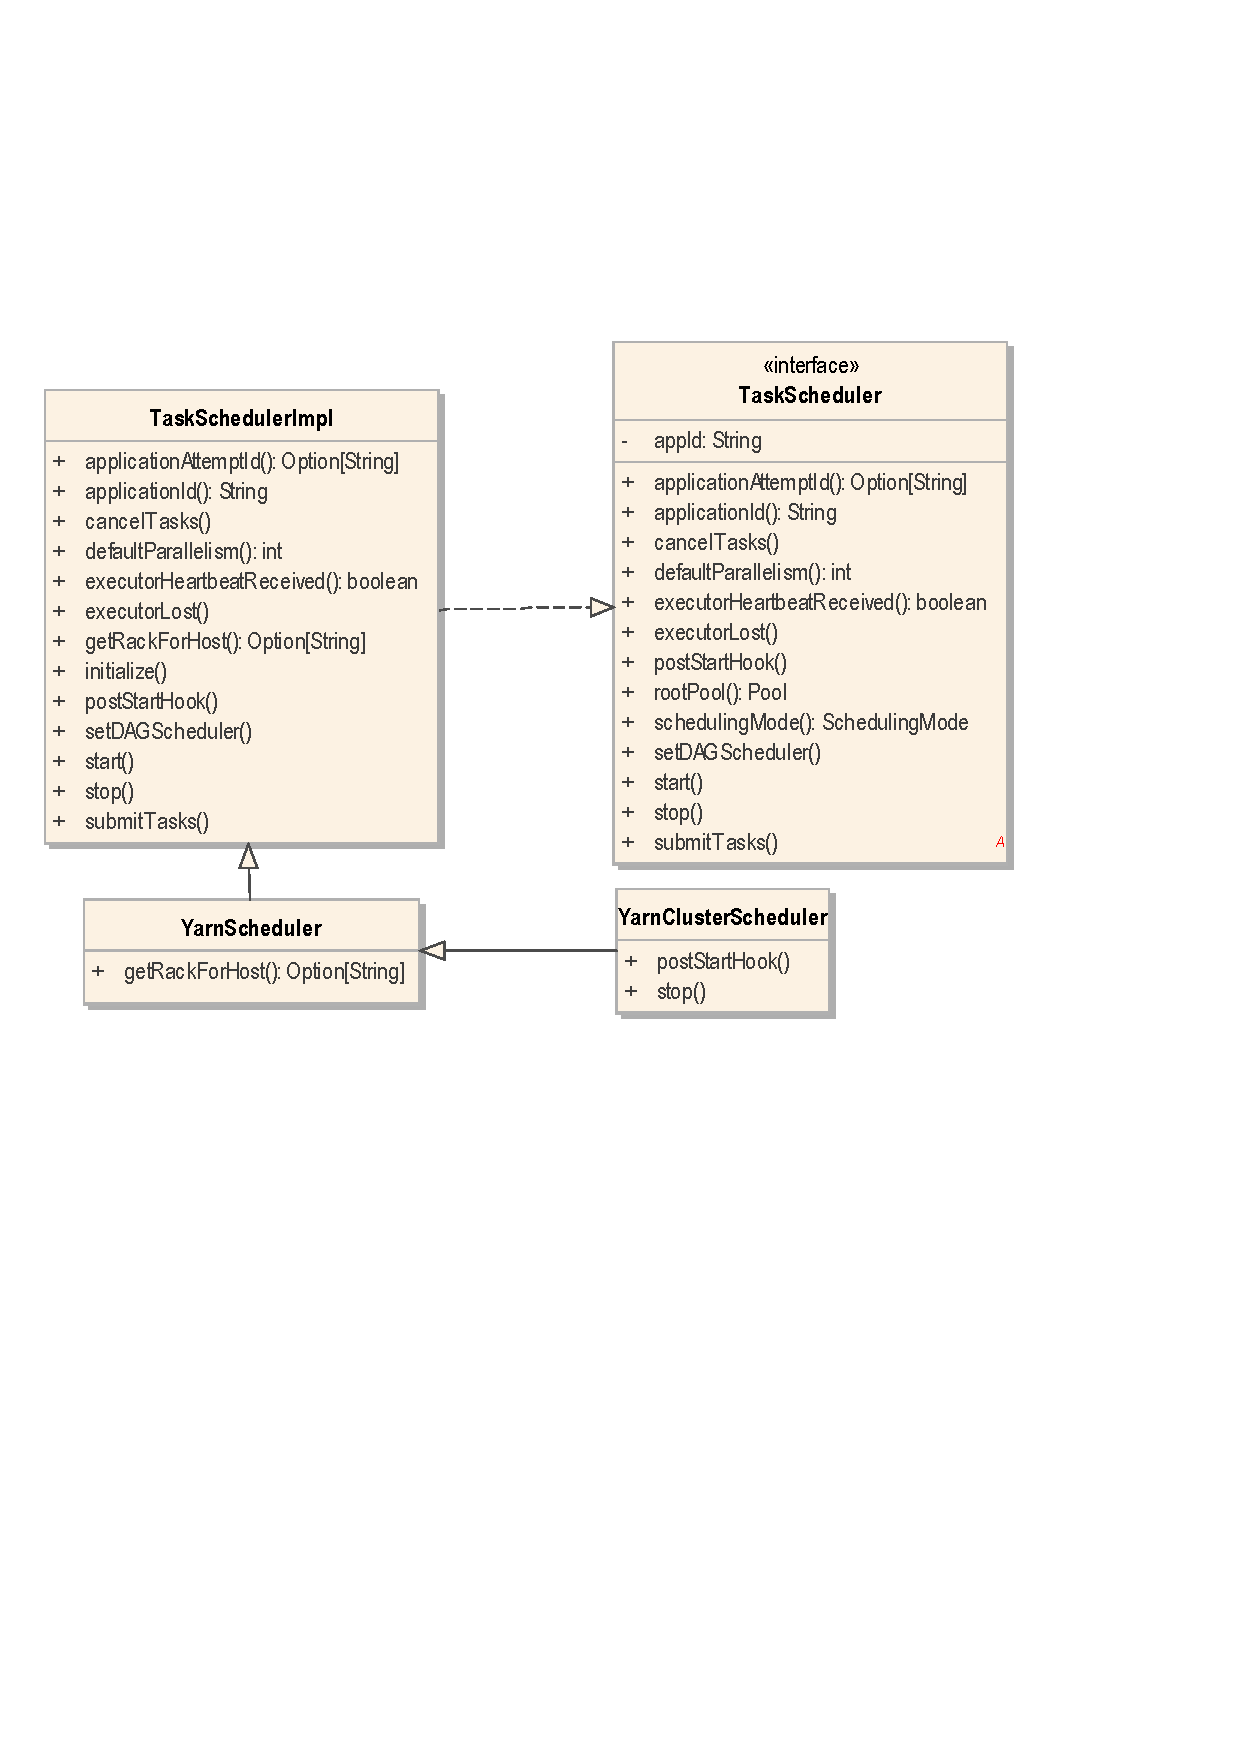
\includegraphics[width=\textwidth]{figures/YarnScheduler.pdf}
		\caption{YarnScheduler类图}
		\label{fig:YarnScheduler}
	\end{figure}

程序\ref{inputPrg:matchyarnclusrer}中倒数第二行代码,Scheduler调用initialize方法对backend进行绑定,我们可以从类图\ref{fig:YarnScheduler}看到实际上是调用了TaskSchedulerImpl\#initialize()方法,此方法代码很简短,指定JOb的调度模式,如程序\ref{inputPrg:taskschedulerimpl}所示
\begin{codeInput}{Scala}{调度器初始化实现}{taskschedulerimpl}
def initialize(backend: SchedulerBackend) {
  this.backend = backend
  rootPool = new Pool("", schedulingMode, 0, 0)
  schedulableBuilder = {
    schedulingMode match {
      case SchedulingMode.FIFO =>
      new FIFOSchedulableBuilder(rootPool)
      case SchedulingMode.FAIR =>
        new FairSchedulableBuilder(rootPool, conf)
      }
    }
    schedulableBuilder.buildPools()
}
\end{codeInput}


此方法最重要的作用就是将Scheduler和SchedulerBackend进行绑定,并制定Job的调度模式,当然默认情况下为FIFO。

接着执行\_taskScheduler.start(),由类图\ref{fig:YarnScheduler}可知实际上调用的是TaskSchedulerImpl\#start()方法,此方法代码如程序\ref{inputPrg:starttaskscheduler}所示,此方法首先调用YarnClusterSchedulerBackend\#start(),之后判断是否需要检查慢服务。
\begin{codeInput}{Scala}{开启任务调度器}{starttaskscheduler}
override def start() {
  //Yarn-cluster模式下为YarnClusterSchedulerBackend
  backend.start()	
    if (!isLocal && conf.getBoolean("spark.speculation", false)) {
      speculationScheduler.scheduleAtFixedRate(new Runnable {
        override def run(): Unit = Utils.tryOrStopSparkContext(sc) {
          checkSpeculatableTasks()
        }
      }, SPECULATION_INTERVAL_MS, SPECULATION_INTERVAL_MS, TimeUnit.MILLISECONDS)
    }
}
\end{codeInput}
	\item YarnClusterSchedulerBackend相关
	
	与其相关的类及接口如图\ref{fig:YarnSchedulerBackend}所示
	\begin{figure}[H] 
		\centering
		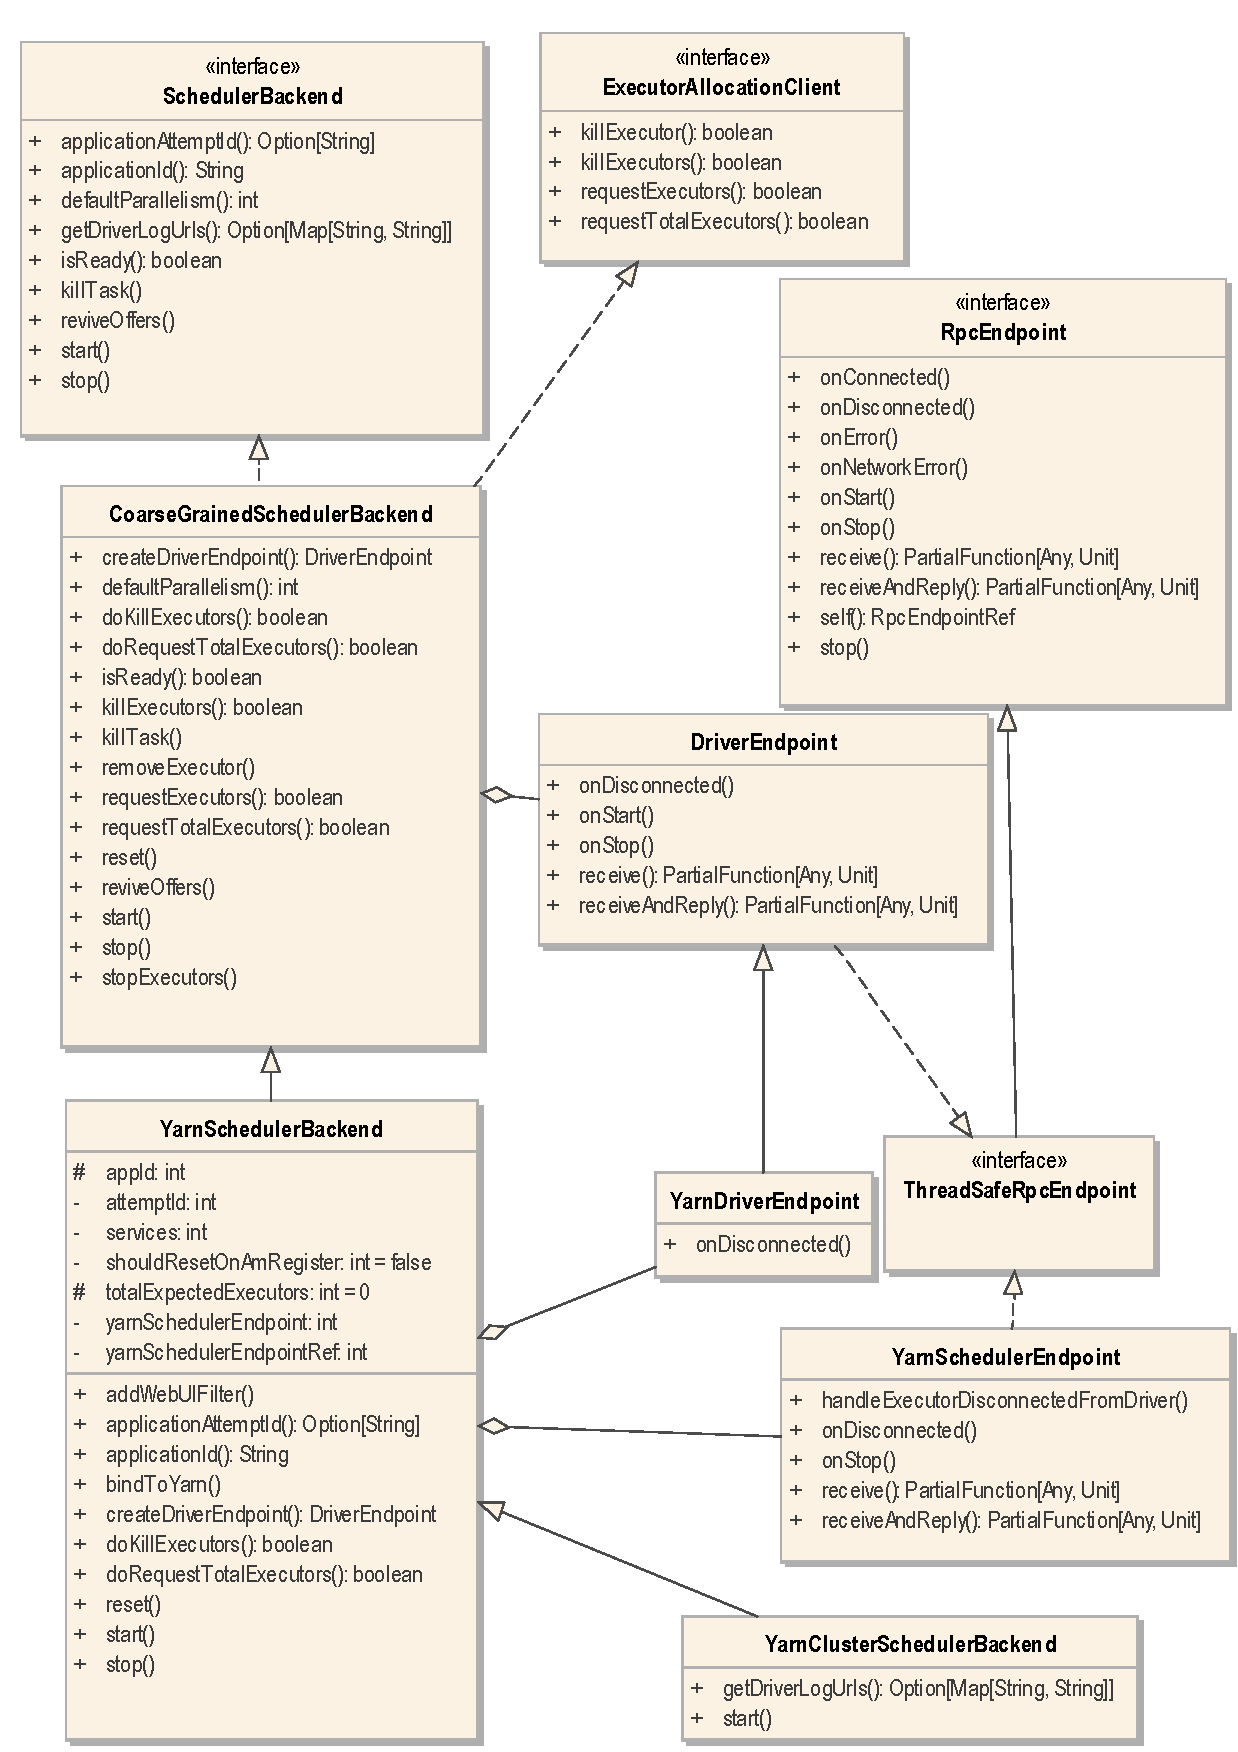
\includegraphics[width=\textwidth]{figures/YarnSchedulerBackend.pdf}
		\caption{YarnSchedulerBackend类图}
		\label{fig:YarnSchedulerBackend}
	\end{figure}
	接着从TaskSchedulerImpl\#start()方法,该方法中第一行即执行YarnClusterSchedulerBackend\#start(),作用为,将appid和attemptId绑定到Yarn上;调用父类的YarnSchedulerBackend\#start()方法。
	
	
	YarnSchedulerBackend\#start()方法:验证appid是否已经定义;Yarn-Cluster模式下,绑定SchedulerExtensionServiceBinding;调用父类CoarseGrainedSchedulerBackend\#start()方法;
	
	CoarseGrainedSchedulerBackend\#start()方法如程序\ref{inputPrg:CoarseGrainedScheduler}所示
	\begin{codeInput}{Scala}{开启CoarseGrainedScheduler}{CoarseGrainedScheduler}
  override def start() {
    val properties = new ArrayBuffer[(String, String)]
    for ((key, value) <- scheduler.sc.conf.getAll) {
      if (key.startsWith("spark.")) {
        properties += ((key, value))
      }
    }		
    // TODO (prashant) send conf instead of properties
    driverEndpoint = rpcEnv.setupEndpoint(ENDPOINT_NAME, createDriverEndpoint(properties))
}
\end{codeInput}

程序\ref{inputPrg:CoarseGrainedScheduler}中RPC在SparkContext\#createSparkEnv函数调用里,具体函数实现流程如图\ref{fig:RPCinitialize}所示。
\begin{figure}[H] 
	\centering
	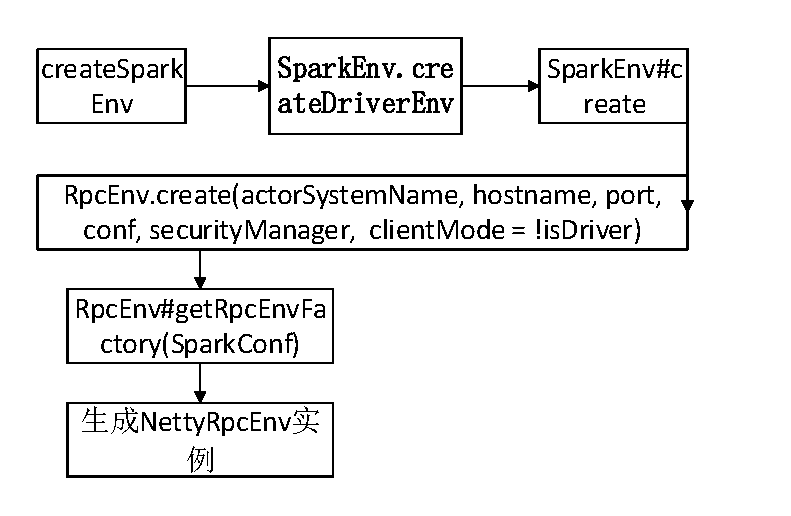
\includegraphics[scale=0.9]{figures/RPCinitialize.pdf}
	\caption{RPC建立过程}
	\label{fig:RPCinitialize}
\end{figure}

流程图\ref{fig:RPCinitialize}可以看出SparkRPC是通过工厂模式反射生成NettyRpcEnv实例。那么CoarseGrainedSchedulerBackend\#start()最后一行就执行的是NettyRpcEnv\#setupEndpoint(),接着执行Dispatcher\#registerRpcEndpoint(),最后就返回了NettyRpcEndpointRef。
\end{enumerate}
\subsection{DAG调度器}
DAGScheduler用于构建Job阶段,将用户应用的DAG划分为不同的Stage,其中Stage由可以并发控制的一组Task构成,这些Task逻辑上完全相同,只是运行在不同的数据分区上。具体的内部实现原理会在Job构建章节中进行讲述。DAGScheduler的数据结构主要维护jobId和stageId的关系、Stage、ActiveJob,以及缓存的RDD的partitions的位置信息。DAGScheduler的数据结构如程序\ref{inputPrg:dagscheduler}所示
\begin{codeInput}{Scala}{DAG调度器数据结构}{dagscheduler}
  private[scheduler] val nextJobId = new AtomicInteger(0)
  private[scheduler] def numTotalJobs: Int = nextJobId.get()
  private val nextStageId = new AtomicInteger(0)
  private[scheduler] val jobIdToStageIds = new HashMap[Int, HashSet[Int]]
  private[scheduler] val stageIdToStage = new HashMap[Int, Stage]
  private[scheduler] val shuffleToMapStage = new HashMap[Int, ShuffleMapStage]
  private[scheduler] val jobIdToActiveJob = new HashMap[Int, ActiveJob]
  // Stages we need to run whose parents aren't done
  private[scheduler] val waitingStages = new HashSet[Stage]
  // Stages we are running right now
  private[scheduler] val runningStages = new HashSet[Stage]
  // Stages that must be resubmitted due to fetch failures
  private[scheduler] val failedStages = new HashSet[Stage]
  private[scheduler] val activeJobs = new HashSet[ActiveJob]
\end{codeInput}


在初始化DAGScheduler的时候,会调用eventProcessLoop\#start(),这个用于创建子线程一直运行的事件监听线程。其调用过程如下图\ref{fig:eventListener}所示
\begin{figure}[H] 
	\centering
	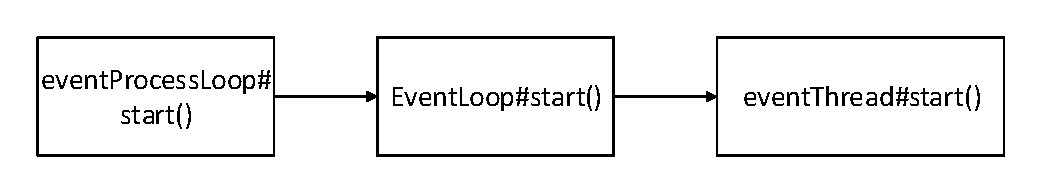
\includegraphics[width=\textwidth]{figures/eventListener.pdf}
	\caption{事件监听开启流程}
	\label{fig:eventListener}
\end{figure}

事件线程运行代码如程序\ref{inputPrg:eventListener}所示
\begin{codeInput}{Scala}{事件监听线程}{eventListener}
private val eventThread = new Thread(name) {
  setDaemon(true)	
  override def run(): Unit = {
    try {
      while (!stopped.get) {
        val event = eventQueue.take()
          try {
            onReceive(event)
          } catch {
            case NonFatal(e) => {
              ......
                }
              }
            }
          } catch {
            ......
        }
    }	
}
\end{codeInput}
从程序\ref{inputPrg:eventListener}中可以看出,事件监听器是个后台守护进程,其中运行的线程是一个由while循环组成的结构,其不断的从事件队列中取出事件,然后调用onReceive(event)方法对不同的事件进行模式匹配。这里的onReceive(event)是一个由子类实现的方法,如程序\ref{inputPrg:onReveive}所示
\begin{codeInput}{Scala}{DAGSchedulerEventProcessLoop.onReveive}{onReveive}
override def onReceive(event: DAGSchedulerEvent): Unit = {
  val timerContext = timer.time()
  try {
    doOnReceive(event)
  } finally {
    timerContext.stop()
  }
}
\end{codeInput}

程序中运行的是doOnReceive(DAGSchedulerEvent)方法,而这个方法中就包含了对不同事件的模式匹配以及对应着不同的处理方式。